\def\tutdate{16.12.2019}

\documentclass[handout]{beamer}
\usepackage{../templates/beamerthemekit}
%\usepackage{enumitem}

\usepackage[utf8]{inputenc}
\usepackage[T1]{fontenc}
\usepackage[ngerman]{babel}
\usepackage{listings}
\usepackage{hyperref}
\usepackage{graphicx}

\usepackage{amsmath}
\usepackage{amsthm}
\usepackage{amssymb}
\usepackage{polynom}

%\usepackage{ifthen}
%\usepackage{adjustbox} % for \adjincludegraphics

%\usepackage{tikz}
\usepackage{listings}

%\usepackage[]{algorithm2e}

%\usepackage{colortbl}
\usepackage{verbatim}
%\usepackage{alltt}
%\usepackage{changes}

%\usepackage{pdfpages}
%\usepackage{tabularx}

%\usepackage{euler}


\newcommand{\markBlue}[1]{\textcolor{kit-blue100}{#1}}
\newcommand{\markGreen}[1]{\textcolor{kit-green100}{#1}}
\newcommand{\vertspace}{\vspace{.2cm}}

%\newcommand{\#}{\markBlue{#1}}

%\newcommand{\pitem}{\pause\item}
\newcommand{\p}{\pause}

% -- MATH MACROS
\newcommand{\thistheoremname}{}
\newcommand{\G}{\mathbb{Z}}
\newcommand{\B}{\mathbb{B}}
\newcommand{\R}{\mathbb{R}}
\newcommand{\N}{\mathbb{N}}
\newcommand{\Q}{\mathbb{Q}}
\newcommand{\C}{\mathbb{C}}
\newcommand{\Z}{\mathbb{Z}}
\newcommand{\F}{\mathbb{F}}
\newcommand{\mi}{\mathrm{i}}
\renewcommand{\epsilon}{\varepsilon}
\newcommand{\okalk}{\mathscr{O}}


\newenvironment<>{taskblock}[1]{%
	\setbeamercolor{block title}{fg=kit-orange15,bg=kit-orange100}
	\setbeamercolor{block body}{fg=black,bg=kit-orange30}%
	\begin{block}#2{#1}}{\end{block}}

\setbeamertemplate{enumerate items}[default]

% Aussagenlogik Symbole
\newcommand{\W}{w}
\renewcommand{\F}{f}

% Kodierung
\newcommand{\frepr}{\textbf{repr}}
\newcommand{\fRepr}{\textbf{Repr}}
\newcommand{\fZkpl}{\textbf{Zkpl}}
\newcommand{\fbin}{\textbf{bin}}
\newcommand{\fdiv}{\textbf{ div }}
\newcommand{\fmod}{\textbf{ mod }}

% Speicherabbild
\newenvironment{memory}{\begin{tabular}{r | l}Adresse&Wert\\\hline\hline}{\end{tabular}}
\newcommand{\memrow}[2]{#1 & #2 \\\hline}

% Praedikatenlogik
\newcommand{\objequiv}{\stackrel{\cdot}{=}}
\newcommand{\pval}{val_{D,I,\beta}}

% Neue Befehle
\newcommand{\ip}{\pause} % inline pause, für mitten im satz
\newcommand{\pitem}{\pause\item} % für aufzählungen
\newcommand{\bp}{\pause} % block pause, für zwischen blöcken
\title[Grundbegriffe der Informatik]{ICPC\\Gruppe 2}
\date{\tutdate}
\subtitle{\tutTitle}
\author{Elias Schaut, Dennis Kobert, Niklas Kniep, Lam Vo, Ilia Bozhinov}

\institute{}

\titleimage{bg}
%\titleimage{bg-advent}

%
\ifthenelse{\equal{\compiletype}{livebeamer}}
	{
		\def\livebeamermode{1}
	}{}

\ifthenelse{\equal{\compiletype}{print}}
	{
		\def\printmode{1}
	}{}

\setbeamercovered{invisible}

%\usepackage[citestyle=authoryear,bibstyle=numeric,hyperref,backend=biber]{biblatex}
%\addbibresource{templates/example.bib}
%\bibhang1em

	
\def\tutTitle{Algorithmen}
\begin{document}

\selectlanguage{ngerman}

%title page
\begin{frame}
	\titlepage
\end{frame}

\section{Algorithmen}
\begin{frame}{Algorithmen}
	\begin{itemize}
		\pitem Es existiert eine \textbf{endliche} Beschreibung
		\pitem Die Anweisungen sind elementar
		\pitem Es wird zu einer beliebig großen, aber \textbf{endlichen} Eingabe eine \textbf{endliche} Ausgabe berechnet
		\pitem Es finden \textbf{endlich} viele Schritte statt (der Algorithmus terminiert)
		\pitem Deterministisch (bei mehrmaliger Ausführung kommt immer das selbe raus)
	\end{itemize}
\end{frame}

\subsection{Pseudocode}
\begin{frame}{Hier verwendeter Pseudocode}
	\begin{itemize}
		\pitem Zuweisungssymbol $\leftarrow$
		\pitem Schlüsselwörter für Verzweigungen \textbf{if, then, else, fi}
		\pitem Schlüsselwörter für Schleifen \textbf{while, do, od, for, to}
		\pitem Symbole für Konstanten, Funktionen und Relationen
	\end{itemize}
\end{frame}

\begin{frame}
	Eine \textbf{if}-Verzweigung\\
	\vspace{0.2cm}
	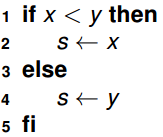
\includegraphics[scale=0.6]{images/if.png}\\
	\vspace{0.2cm}\p
	Eine \textbf{while}-Schleife\\
	\vspace{0.2cm}
	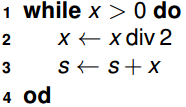
\includegraphics[scale=0.6]{images/while.png}\\
	\vspace{0.2cm}\p
	Eine \textbf{for}-Schleife\\
	\vspace{0.2cm}
	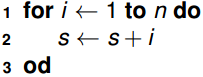
\includegraphics[scale=0.6]{images/for.png}
\end{frame}

\begin{frame}{Was kann man mit Algorithmen machen?}
	\begin{itemize}
		\pitem Komplexe Algorithmen mit Pseudocode definieren zu Sortierung, Graphen, Datenstrukturen\ip, im Modul \markBlue{Algorithmen I}
		\pitem Laufzeitanalyse von Algorithmen\ip, später.
		\pitem Korrektheitsbeweise\ip, jetzt.
	\end{itemize}
\end{frame}

\begin{frame}{Korrektheitsbeweise}
	\ip Wie findet man heraus, ob ein Algorithmus korrekt funktioniert?
	\begin{itemize}
		\pitem Durch den Beweis von Zusicherungen, die an bestimmten Stellen des Algorithmus gelten.
	\end{itemize}

	\vertspace

	\bp Was sind Zusicherungen?
	\begin{itemize}
		\pitem prädikatenlogische Formeln, die Aussagen über (Zusammenhänge zwischen) Variablen machen
	\end{itemize}
\end{frame}



%	\begin{frame}
%	\textbf{Beispiel}\\
%	Was ist hier die Schleifeninvariante?\\
%	\vspace{0.1cm}
%		Seien $a,b \in \mathbb{N}_0$\\
%		$x \leftarrow b$\\
%		$x \leftarrow a$\\
%		$while$ $y \neq 0$\\
%		do \\
%		\hspace{0.4cm} $y \leftarrow y - 1$\\
%		\hspace{0.4cm} $x \leftarrow x + 1$\\
%		od
%	\end{frame}


\subsection{Das Hoare-Kalkül}
\begin{frame}{Das Hoare-Tripel}
	\p
	
	\begin{block}{Definition}
		$\{P\}S\{Q\}$ heißt Hoare-Tripel. \ip Dabei gilt:
		\begin{itemize}
			\pitem S ist ein Programmstück im Pseudocode
			\pitem P und Q sind Zusicherungen
		\end{itemize}
	\end{block}
	\begin{itemize}
		\pitem P nennt man Vorbedingung, Q Nachbedingung
		\pitem Prädikatenlogische Formeln
		\pitem Beispiel (Vorausblick): $\{x \objequiv  1 \} x \leftarrow x + 1 \{x \objequiv 2\}$
		\pitem Meistens in jeder Zeile nur eine Zeile Code oder ein Zusicherungsblock
	\end{itemize}
\end{frame}

\begin{frame}{Das Hoare-Tripel}
	\begin{block}{Gültigkeit von Hoare-Tripeln}
		$\{P\}S\{Q\}$ ist gültig, wenn für jede gültige Interpretation $(D, I)$ und Variablenbelegung $\beta$ gilt:\\\bp
		Aus 
		\begin{itemize}
			\pitem $val_{D, I, \beta}(P) = w$
			\pitem $\beta'$ ist Variablenbelegung nach Ausführung von $S$
		\end{itemize}
		\ip folgt $val_{D, I, \beta'}(Q) = w$
	\end{block}
\end{frame}

\begin{frame}{Zuweisung}
	\begin{block}{Axiom HT-A}
		\begin{itemize}
			\pitem Sei $x \leftarrow E$ eine Zuweisung
			\pitem $Q$ eine Nachbedingung von $x \leftarrow E$ und
			\pitem $\sigma_{\{x/E\}}$ kollisionsfrei für Q
		\end{itemize}
		\p Dann ist $\sigma_{\{x/E\}}(Q) x \leftarrow E\{Q\}$ ein gültiges Hoare-Tripel
	\end{block}\p
	\textbf{Bemerkung}\\
	\begin{itemize}
		\pitem $\sigma_{\{x/E\}}$ ist die Substitution von $x$ mit $E$
		\pitem Bei Anwendung der Regel rückwärts vorgehen
	\end{itemize}
\end{frame}

\begin{frame}
	\textbf{Beispiel}\\
	Betrachte die Zuweisung \\
	$x \leftarrow x +1$\\
	und die Nachbedingung\\
	$\{x \dot = 1\}$\\
	\ip Nach HT-A gilt\\
	\pause
	$\{x+1 \dot = 1\}$ $ x \leftarrow x + 1$ $ \{x \dot = 1\}$ ist ein gültiges Hoare-Tripel.
\end{frame}

\begin{frame}{Ableitungsregeln: HT-E}
	\begin{itemize}
		\item Verstärkung der Vorbedingung
		\item Abschwächung der Nachbedingung
	\end{itemize}\p
	\begin{block}{HT-E}
		Wenn $\{P\}S\{Q\}$ ein gültiges Hoare-Tripel ist und $P' \vdash P$ und $Q \vdash Q'$ gelten, dann folgt:\\
		\pause
		$\{P'\}S \{Q'\}$ ist ein gültiges Hoare-Tripel.
	\end{block}
	\p\textbf{Bemerkung}\\
	$B \vdash A :\Leftrightarrow$ Aussage $A$ ist syntaktisch aus Aussage $B$ ableitbar
\end{frame}

\begin{frame}
	\textbf{Beispiel}\\
	Angenommen es sei $\{y > 3\}$ $x \leftarrow y-1$ $\{x > 1\}$ ein gültiges Hoare-Tripel.\\
	Es gilt $\{(y>4)\} \vdash \{(y>3)\} $ und $\{(x>1)\} \vdash \{(x>0)\} $.\\
	Also folgt nach HT-E:\\
	\pause
	$\{y > 4\}$ $x \leftarrow y-1$ $\{x > 0\}$ ist ein gültiges Hoare-Tripel.\\
	\pause
	\vertspace
	\textbf{Bemerkung}\\
	Es müssen sich nicht unbedingt beide Bedingungen ändern! \\
	Aus $\{(y>3)\} \vdash \{(y>3)\} $ und $\{(x>1)\} \vdash \{(x>0)\} $ \\folgt nach HT-E auch \\
	$\{y > 3\}$ $x \leftarrow y-1$ $\{x > 0\}$ ist ein gültiges Hoare-Tripel.
\end{frame}

\begin{frame}{Ableitungsregeln: HT-S}
	\p Hintereinanderausführung von durch Hoare-Triple bewiesene Code Segmente sind selbst gültig.\p
	\begin{block}{HT-S}
		Wenn $\{P\}S_1\{Q\}$ und $\{Q\}S_2\{R\}$ gültige Hoare-Tripel sind\ip, dann folgt:\ip $\{P\}S_1; S_2\{R\}$ ist ein gültiges Hoare-Tripel. 
	\end{block}
	\p\textbf{Bemerkung}\\
	";"  \space trennt hier zwei Programmstücke
\end{frame}

\begin{frame}
	\textbf{Beispiel}\\
	Angenommen es seien $\{y > 3\}$ $x \leftarrow y-1$ $\{x > 1\}$ und \\
	$\{x > 1\}$ $z \leftarrow x-1$ $\{z > -1\}$ gültige Hoare-Tripel.\\
	\ip Dann folgt nach HT-S:\\
	\pause
	$\{y > 3\}$ $x \leftarrow y-1; z \leftarrow x-1$ $\{z > -1\}$ ein gültiges Hoare-Tripel.
\end{frame}

\begin{frame} {Bedingte Anweisungen}\p
	\begin{block}{HT-I}
		Wenn $\{P \land B\}S_1\{Q\}$ und $\{P \land \lnot B\}S_2\{Q\}$ gültige Hoare-Tripel sind\ip, dann folgt:\\
		
		\vertspace
		\quad$\{P\}$\\
		\qquad\textbf{if} $B$ \textbf{then} $S_1$ \\
		\qquad\textbf{else} $S_2$\\
		\qquad\textbf{fi}\\
		\quad$\{Q\}$\\
		\vertspace
		
		
		ist ein gültiges Hoare-Tripel.
	\end{block}
\end{frame}

\begin{frame}{Beispiel}
	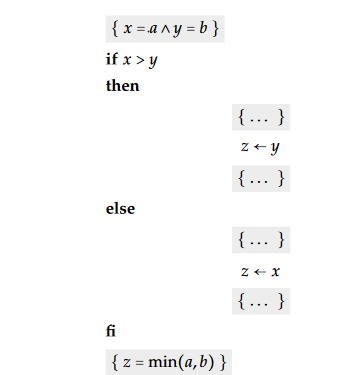
\includegraphics[scale=0.6]{images/if_fi.PNG}
\end{frame}		

\begin{frame}{Beispiel}
	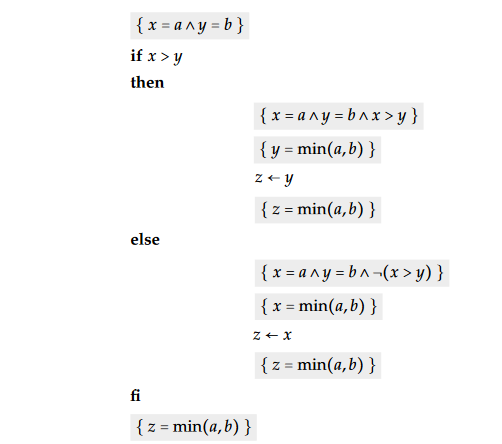
\includegraphics[scale=0.6]{images/if_fi_loes.PNG}
\end{frame}		

%\begin{frame}{Weiteres Beispiel}
%Sei $p$ eine Person, $betrunken(p)$ ein einstelliges Prädikat mit $betrunken(p) = wahr %:\Leftrightarrow getrunkeneGl"uhweins \objequiv 20$.
%\begin{algorithm}
%	$\{getrunkeneGl"uhweins = 0\}$
%	\While{$\lnot betrunken(p)$}{$getrunkeneGl"uhweins \leftarrow getrunkeneGl"uhweins + 1$}
%\end{algorithm}
%\end{frame}

\begin{frame} {Schleifen}
	\begin{block}{HT-W}
		Wenn $\{I \land B\}S\{I\}$ ein gültiges Hoare-Tripel ist\ip, dann folgt:\\\ip
		
		\vertspace
		$\{I\}$\\
		\textbf{while} $B$
		\textbf{do} $S$ \\
		\textbf{od}\\
		$\{I \land \lnot B\}$\\
		\vertspace
		
		ist ein gültiges Hoare-Tripel.
	\end{block}
\end{frame}

\begin{frame}{Schleifeninvariante}
	\begin{itemize}
		\pitem Eine spezielle Zusicherung
		\pitem Schleifeninvarianten müssen \textbf{vor}, \textbf{während} und \textbf{nach} jedem Schleifendurchlauf gelten
		\pitem Garantiert, dass die Schleife nicht während einem beliebigen Durchlauf ``kaputt'' geht.
		%\pitem Sie \textbf{müssen nicht} während des Schleifendurchlaufs gelten (können aber)
	\end{itemize}
\end{frame}

\begin{frame}
	\textbf{Beispiel}\\
	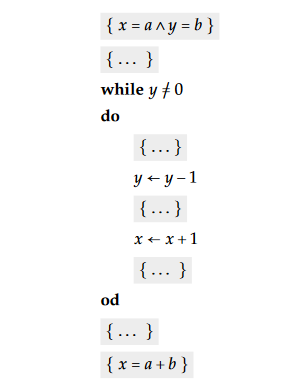
\includegraphics[scale=0.7]{images/do_od.PNG}
\end{frame}

\begin{frame}
	\textbf{Beispiel}\\
	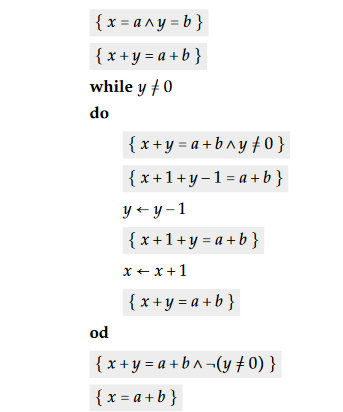
\includegraphics[scale=0.7]{images/do_od_loes.png}
\end{frame}

\begin{frame}
    Bestimmt für den folgenden Algorithmus was er berechnet und eine 
Schleifeninvariante: \\
$\{a \in \N_+, b \in \N_+\}$ \\
$X_0 \leftarrow a$ \\
$Y_0 \leftarrow b $\\
$P_0 \leftarrow 1 $\\
$\alpha_0 \leftarrow X_0 mod  2$ \\
$n \leftarrow 1 + \lceil log_2 a \rceil $\\
$for i \leftarrow 0$ to $n-1 do $ \\
\hspace{5mm}
$P_{i+1} \leftarrow P_i * {Y_i}^{\alpha_i}$ \\
\hspace{5mm}
$X_{i+1} \leftarrow X_i div 2$ \\
\hspace{5mm}
$Y_{i+1} \leftarrow {Y_i}^2$ \\
\hspace{5mm}
$\alpha_{i+1} \leftarrow X_{i+1} mod 2$ \\
od 
\newline \newline
Tipp: Beispieleingabe $a = 5$ und $b = 2$
\end{frame}



\begin{frame}
	
\includegraphics[width=\linewidth]{../images/thatsall.png}
\end{frame}


\end{document}
